\subsection{Quantum Random Number Generator}

Quantum Random Number Generation (QRNG) harnesses the inherent indeterminacy of quantum mechanics to produce random sequences theoretically unpredictable by classical means. At its core, QRNG utilizes qubits which, through the principle of superposition, can represent multiple states simultaneously until a measurement is performed. This act of measurement is pivotal, compelling a qubit to collapse from its superposition into a definite classical state (0 or 1), with the specific outcome governed by quantum probabilities, forming the basis of true randomness.

The translation of these quantum mechanical principles into a practical random bit stream involves a carefully orchestrated process. It begins with the precise preparation of quantum states specifically designed to maximize outcome uncertainty. Subsequent interactions with these prepared states, followed by their measurement, yield a sequence where each outcome, dictated by the probabilistic nature of quantum collapse, contributes a bit to the forming random sequence.

The quantum random number generation (QRNG) methodology implemented, which makes use of code developed by Gehad Salem Fekry, software engineer and quantum researcher and publicly available on GitHub (\url{https://github.com/GehadSalemFekry/qrng/}), begins with the construction of a quantum circuit comprising $N$ qubits, where $N$ dictates the length of the random bit string to be generated. Each qubit is individually subjected to a Hadamard (H) gate operation. This crucial step transforms the qubit from a definite initial state into an equal superposition of the computational basis states $|0\rangle$ and $|1\rangle$, described by the state vector $\frac{1}{\sqrt{2}}(|0\rangle + |1\rangle)$. Consequently, upon measurement, each qubit has an equal probability of collapsing to either 0 or 1, providing the fundamental source of randomness. The collective measurement of all $N$ qubits yields a single $N$-bit string derived from these inherently probabilistic quantum events.

For the practical realization of these random bits, the constructed quantum circuit is executed on a quantum backend, accessed via the Qiskit Runtime Service which can select an operational quantum processor or a simulator. Prior to execution, the circuit undergoes a transpilation process, adapting it to the specific gate set and connectivity constraints of the target backend. The transpiled circuit is then run for a significant number of shots (e.g., 5000 as specified in the implementation), with the `memory=True` option enabling the retrieval of the exact bit string outcome from each individual shot. These collected bit strings constitute the raw output of the QRNG process.


\subsection{Randomness Beacon Architecture}

As defined by the NIST, a \textbf{Randomness Beacon} is a service that provides periodic pulses of random numbers. These pulses are timestamped, hash-chained, and signed (Kelsey, Brand\~{a}o, T. A, Peralta, Booth, 2019).

A beacon is composed of:
\begin{itemize}
    \item An \textbf{engine}, which is a computer with clear physical boundaries where the pulses are formed and where the ``beacon app'' is run.
    \item A \textbf{frontend} through which users can access the beacon's information, including the latest pulse as well as the history of all pulses ever generated by the beacon.
    \item An \textbf{HSM} (Hardware Security Module), independent from the engine, used for cryptographic operations.
    \item At least \textbf{two RNGs}, with at least one being independent from the beacon's engine.
\end{itemize}

\begin{figure}[h]
    \centering
    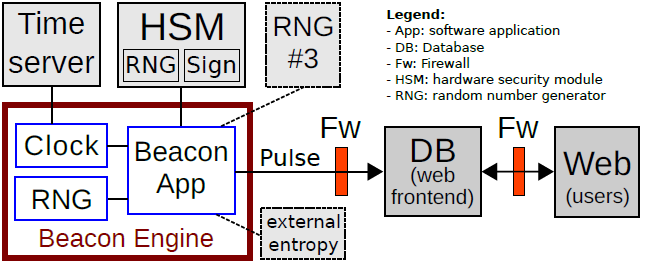
\includegraphics[width=\columnwidth]{images/ArchitectureNISTBeacon.PNG}
    \caption{The general layout of a Randomness Beacon (Kelsey, Brand\~{a}o, T. A, Peralta, Booth, 2019).}
    \label{fig:beacon-architecture}
\end{figure}

The \textbf{NIST Randomness Beacon} is one such beacon; it is a public source of periodical randomness. It produces a 512-bit pulse every minute and makes it available at the established timestamp for anyone to use. For the purposes of this research, we focus on its RNGs. The NIST Beacon currently uses three:

\begin{itemize}
    \item the Intel RNG included in the engine,
    \item a QRNG based on photon detection developed by NIST,
    \item and the hardware RNG inside the HSM (Kelsey, 2018).
\end{itemize}

The model and specifics of the HSM used are not disclosed, so we focus on the other two.

\subsection{The Intel RNG}
The Intel RNG is a DRNG integrated into many Intel CPUs. It utilizes the RDRAND and RDSEED instructions, which are part of the Intel 64 architecture, and implements them directly on the hardware. Its architecture includes an entropy source, a conditioner to convert entropy into random numbers, and two parallel outputs: a DRBG and an ENRNG (Mechalas, 2018).

\begin{figure}[h]
    \centering
    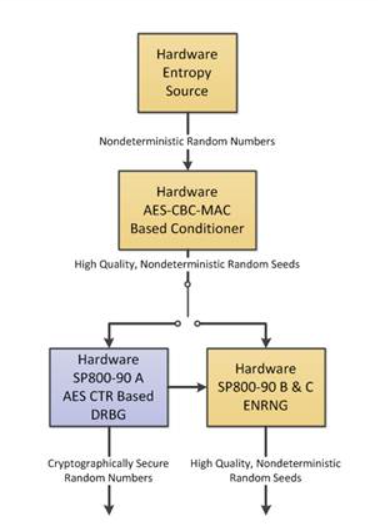
\includegraphics[width=\columnwidth]{images/IntelDRNPipeline.PNG}
    \caption{Intel’s DRNG Component Architecture (Mechalas, 2018).}
    \label{fig:beacon-architecture}
\end{figure}
The entropy source measures thermal noise within the silicon of the CPU and outputs randomness as a binary stream at a rate of 3 GHz.

\subsection{The QRNG}
The QRNG based on photon detection is described by Zhang, Yanbao, Hsin-Pin Lo, Alan Mink, Takuya Ikuta, Toshimori Honjo, Hiroki Takesue, and William J. Munro in their publication \textit{A Simple Low-Latency Real-Time Certifiable Quantum Random Number Generator} (Zhang et al., 2021). It operates as follows:

\begin{quote}
At each trial a horizontally polarized single photon is emitted from a source, and then measured randomly along either the X-basis (diagonal/anti-diagonal polarization basis) to generate a random bit or the Z-basis (horizontal/vertical polarization basis) to verify the prepared state.
\end{quote}

In practice, the NIST QRNG measures photons prepared in a superposition of two time bins---early ($t_e$) and late ($t_l$)---a technique known as \textbf{time-bin encoding}. Photons pass through an unbalanced Mach-Zehnder interferometer (MZI), where the path-length difference matches the separation between $t_e$ and $t_l$. This results in the photon being detected at $t_e$, $t_l$, or the interference slot $t_m$.

\begin{itemize}
    \item Detection at $t_e$ or $t_l$ implies no interference: Z-basis measurement (which time bin).
    \item Detection at $t_m$ implies interference: X-basis measurement (superposition).
\end{itemize}

The basis is chosen passively and randomly, depending on the photon's path through the MZI. The outcomes are fundamentally unpredictable due to quantum mechanics. This combination ensures real-time, certifiable quantum randomness.

\subsection{Hashing of RNG Output}
The NIST Randomness Beacon concatenates the outputs from its RNGs and applies a SHA-512 hash. The resulting hash value becomes the \textit{localRandomValue} of the pulse (Kelsey, 2021).

\subsection{CTR\_DRBG Counter mode Deterministic Random Bit Generator}
\label{sec:counter_mode_deterministic_random_bit_generator}

\begin{quote}
\textbf{CTR\_DRBG (Counter mode Deterministic Random Bit Generator)} is a standardized method for constructing a deterministic random bit generator (PRNG) using a block cipher operating in counter (CTR) mode. This technique is defined in NIST Special Publication 800-90A, titled \textit{``Recommendation for Random Number Generation Using Deterministic Random Bit Generators''}. Essentially, CTR\_DRBG transforms a secure symmetric cipher---such as AES---into a cryptographically strong source of pseudorandom bits. The counter mode ensures that each generated block is unique by systematically incrementing a counter value for each new data request, thus preventing the repetition of output sequences under the same key and seed. This approach is widely used in cryptographic applications requiring high security and reliability in random data generation, such as key generation, initialization vectors, and session tokens.
\end{quote}

